\begin{figure}[b!]
  \vspace{-1.5em}
  \centering
  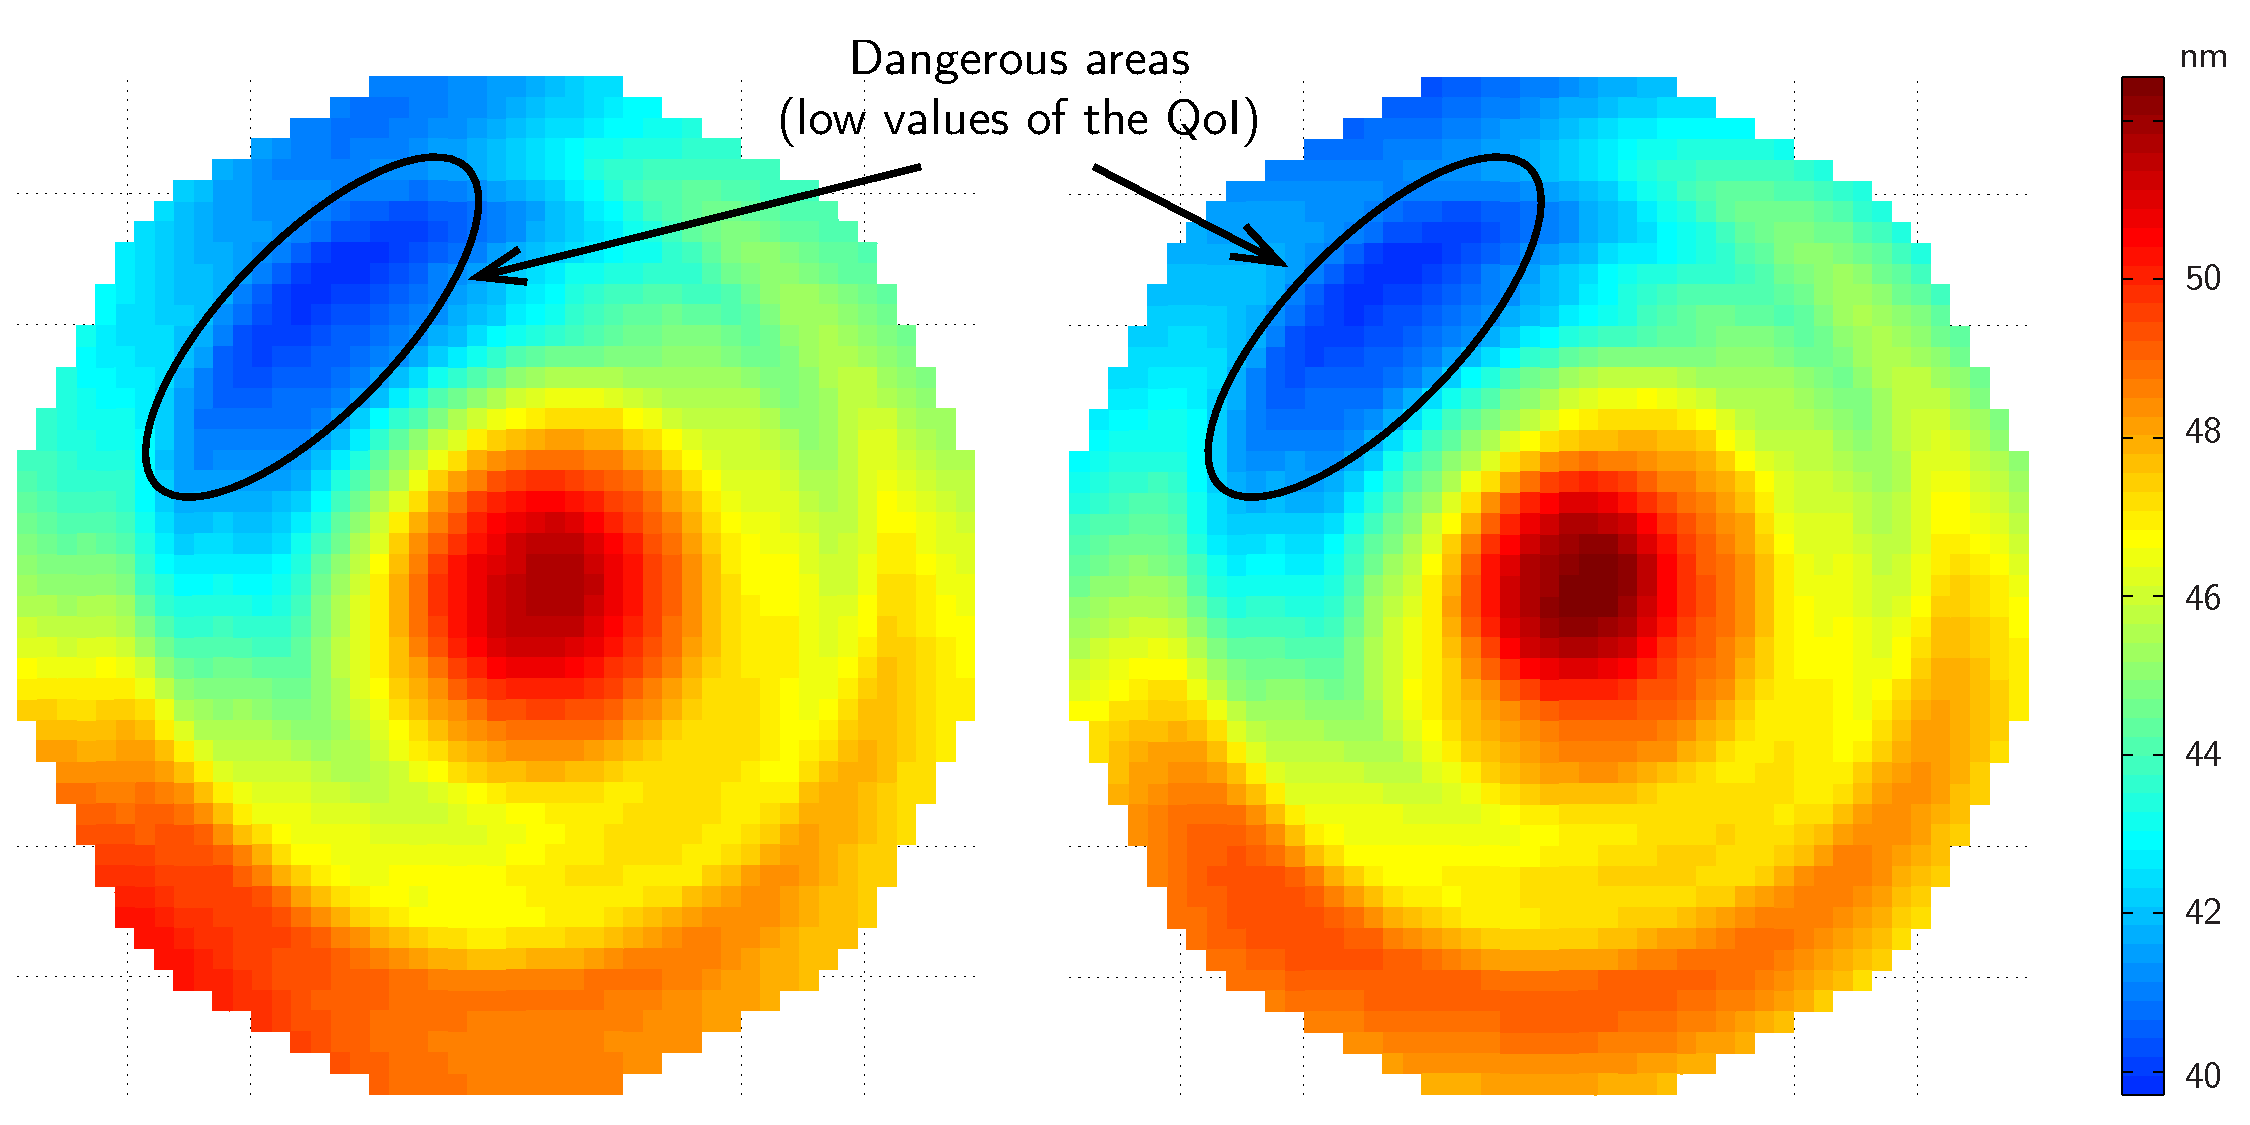
\includegraphics[width=1\linewidth]{include/assets/wafer-qoi.pdf}
  \caption{The true (on the left) and inferred (on the right) distribution of the QoI across the wafer.}
  \flabel{wafer-qoi}
\end{figure}

Let us consider an example that illustrates a particular application of the proposed technique. As previously mentioned, due to process variation, the key parameters that have direct impacts on power and temperature are intrinsically uncertain. Let $\u$ be one of such uncertain quantities; say, the effective channel length. Assume the manufacturing process imposes a lower bound $\u_*$ on the parametrization $\u$. This lower bound separates defective dies ($\u_* > \u$) from those that function properly ($\u_* \leq \u$). Possible actions that one might wish to take with respect to a single die on the wafer are: (a) keep the die if it closely conforms to the specification; (b) throw away the die if it exhibits an unacceptable divergence, due to process variation, from the specification. Let the distribution of $\u$ across the wafer be the one depicted in \fref{wafer-qoi-true} where 316 dies, four cores each, are placed in a $20 \times 20$ grid, and the gradient from navy to dark red represents the transition of $\u$ from low to high values.\footnote{The experimental setup is described in \sref{experimental-results} in details.} A common approach to find this distribution is to deploy adequate test structures on the dies and measure $\u$ directly; then, the corresponding decision can be taken based on the collected information. The problem, however, is that the described procedure is typically expensive to undertake. The technique that we propose and develop in this paper operates on cheap, indirect measurements, denoted by $\Data$, and, therefore, can considerably decrease these costs. The result of an application of our framework to a data set of only 20 die measurements out of 316 is shown in \fref{wafer-qoi-inferred} where the normalized root-mean-square error (NRMSE) is $2.75\%$. Furthermore, the technique can readily be utilized to estimate probabilities of various events, \eg, $\probabilityMeasure(\u_* > \u)$. This fact is especially handy since, in reality, we do not known the true values and, therefore, can reason about our decisions only in terms of probabilities. We can then reformulate our decision rule as follows: (a) keep the die if $\probabilityMeasure(\u_* \leq \u)$ is larger then a certain threshold; (b) throw the die away if $\probabilityMeasure(\u_* > \u)$ is larger then some other threshold. In addition, we can introduce a trade-off action: (c) expose the die to a thorough inspection (\eg, via a test structure) if (a) and (b) cannot be taken. An illustration of this process is given in \fref{wafer-defect} where the threshold is set to two standard deviation below the mean value of $\u$, the circles mark defective dies (the navy areas in \fref{wafer-qoi-true}), and the gradient from light gray to red corresponds to the inferred probability of a die to be defective. It can be seen that the inference accurately detects faulty regions.
\begin{figure}[t!]
  \centering
  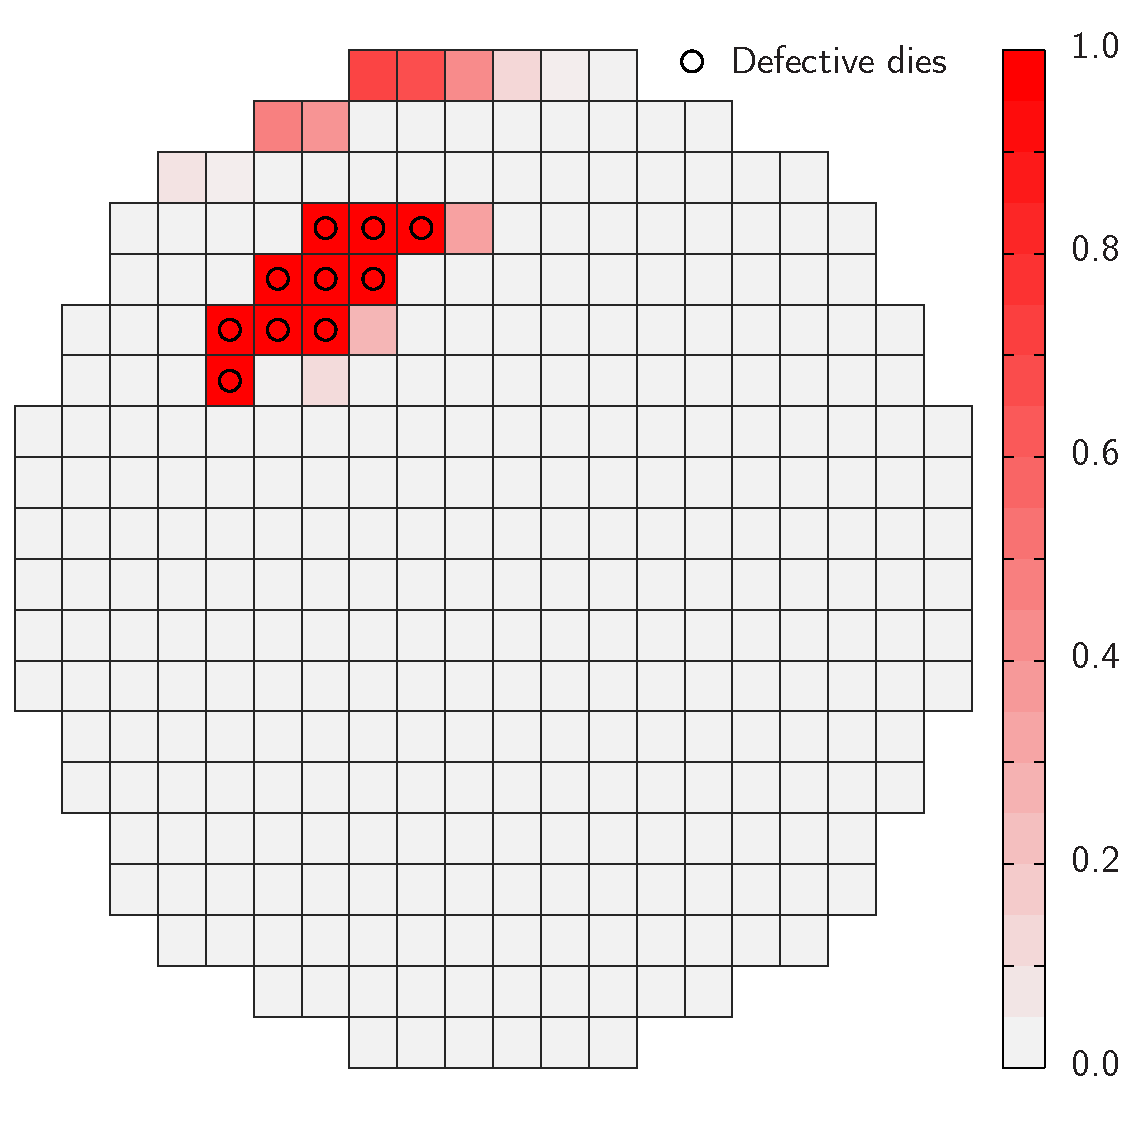
\includegraphics[width=0.7\linewidth]{include/assets/wafer-defect.pdf}
  \caption{Inferred probability of defective dies.}
  \flabel{wafer-defect}
  \vspace{-1.5em}
\end{figure}

